
\section{Other considerations}
\label{sec:considerations}

In this section we present a straightforward generalization of the classic $F$ and $F_1$ to allow other exponents. In Section \ref{subsec:fq} we show that in this generalized class of statistics $F_1$ is indeed optimal. In Section \ref{subsec:params} we discuss the experimental exploration of the full parameter space that guides the formulation of the $F_1$ statistic.

\subsection{Varying the exponent}\label{subsec:fq}
As seen is the previous sections, the change from squaring the differences in the original $F$-test to taking their absolute value with the $F_1$-statistic improved power significantly in the differentially private setting. It is not obvious that switching the exponent from 2 to 1 is optimal --- perhaps some other exponent is superior. An exponent of 0 is clearly horrible, so there must be a local maximum in the power of the statistic for some exponent between 0 and 2.

In order to determine which exponent is in fact optimal, we further generalize the notion of an $F$-test.  We define \sqa and \sqe, which are equivalent to \ssa and \sse except that the summand is raised to the $q^{\text{th}}$ exponent, and we call the resulting statistic $F_q$.  Note that $F_1$ (as defined earlier) is a special case of $F_q$ for $q=1$, and $F_2$ is the standard $F$-statistic.

\begin{definition}[$F_q$] \label{def:Fq} 
Given a database \x with \k groups and \dbsize total entries, define \sqa and \sqe as follows:
%
\begin{equation*}
\sqa(\x) = \sum_{j=1}^k n_j \left\vert \overline{y}_j - \overline{y} \right\vert^q
\end{equation*}
%
\begin{equation*}
\sqe(\x) = \sum_{i=1}^N \left\vert y_i - \overline{y}_{c_i} \right\vert^q
\end{equation*}
%
Then, $F_q$ is defined as
%
\begin{equation*}
F_q(\x) = \frac{\sqa/(\k-1)}{\sqe/(\dbsize-\k)}
\end{equation*}
%
\end{definition}
%%%
We must now create a private approximation of $F_q$ for arbitrary $q$.  To do this, we first bound the sensitivity of the \sqa and \sqe with the following two theorems, the proofs of which can be found in Appendix \ref{sec:fqsensitivity}.
%%%
\begin{theorem}[\sqe Sensitivity] \label{thm:SQEsens} 
The sensitivity of \sqe is bounded above by
\begin{equation*}
2\bigg(\frac{\dbsize}{2}\bigg)^{(1-q)} + 1
\end{equation*}
when $q \in (0,1)$ and
\begin{equation*}
\dbsize - \dbsize\bigg(1-\frac{2}{\dbsize}\bigg)^q +1 
\end{equation*}
when $q\geq 1$. Note that both give an upper bound of 3 when $q=1$.
\end{theorem}


\begin{theorem}[\sqa Sensitivity]\label{thm:SQAsens} The sensitivity of \sqa is bounded above by 
\begin{equation*}
\dbsize\bigg(\frac{3}{\dbsize}\bigg)^q + 1
\end{equation*}
when $q \in (0,1)$ and
\begin{equation*}
\dbsize-\dbsize\bigg(1-\frac{3}{\dbsize}\bigg)^q + 1
\end{equation*}
when $q \geq 1$. Note that both give an upper bound of 4 when $q = 1$.
\end{theorem}


Given these sensitivity bounds, we can calculate a private approximation of $F_q$ for simulated data using the same algorithm as for $F_1$, but with the sensitivities altered according to the choice of $q$.  We can also simulate a reference distribution by adapting Algorithm~\ref{alg:pval}, which was done to construct Figure \ref{fig:fqpower}.  As is clear from these results, in terms of power, the optimal value of $q$ is 1.

We note that in the computation shown in Figure \ref{fig:fqpower}, we don't estimate $\sigma$ using \sqe.  This is because we have not developed an estimator for $\sigma$ that can be computed from \sqe (for $q \ne 1, 2$).  If another value of $q$ had indeed been optimal, the next step would have been to find such an estimator and confirm it was accurate enough to produce acceptable $p$-values.  But since the power cannot possibly improve when switching to an estimated $\sigma$ value, this result is sufficient to show that other values of $q$ need not be considered.


\begin{figure}
\centering
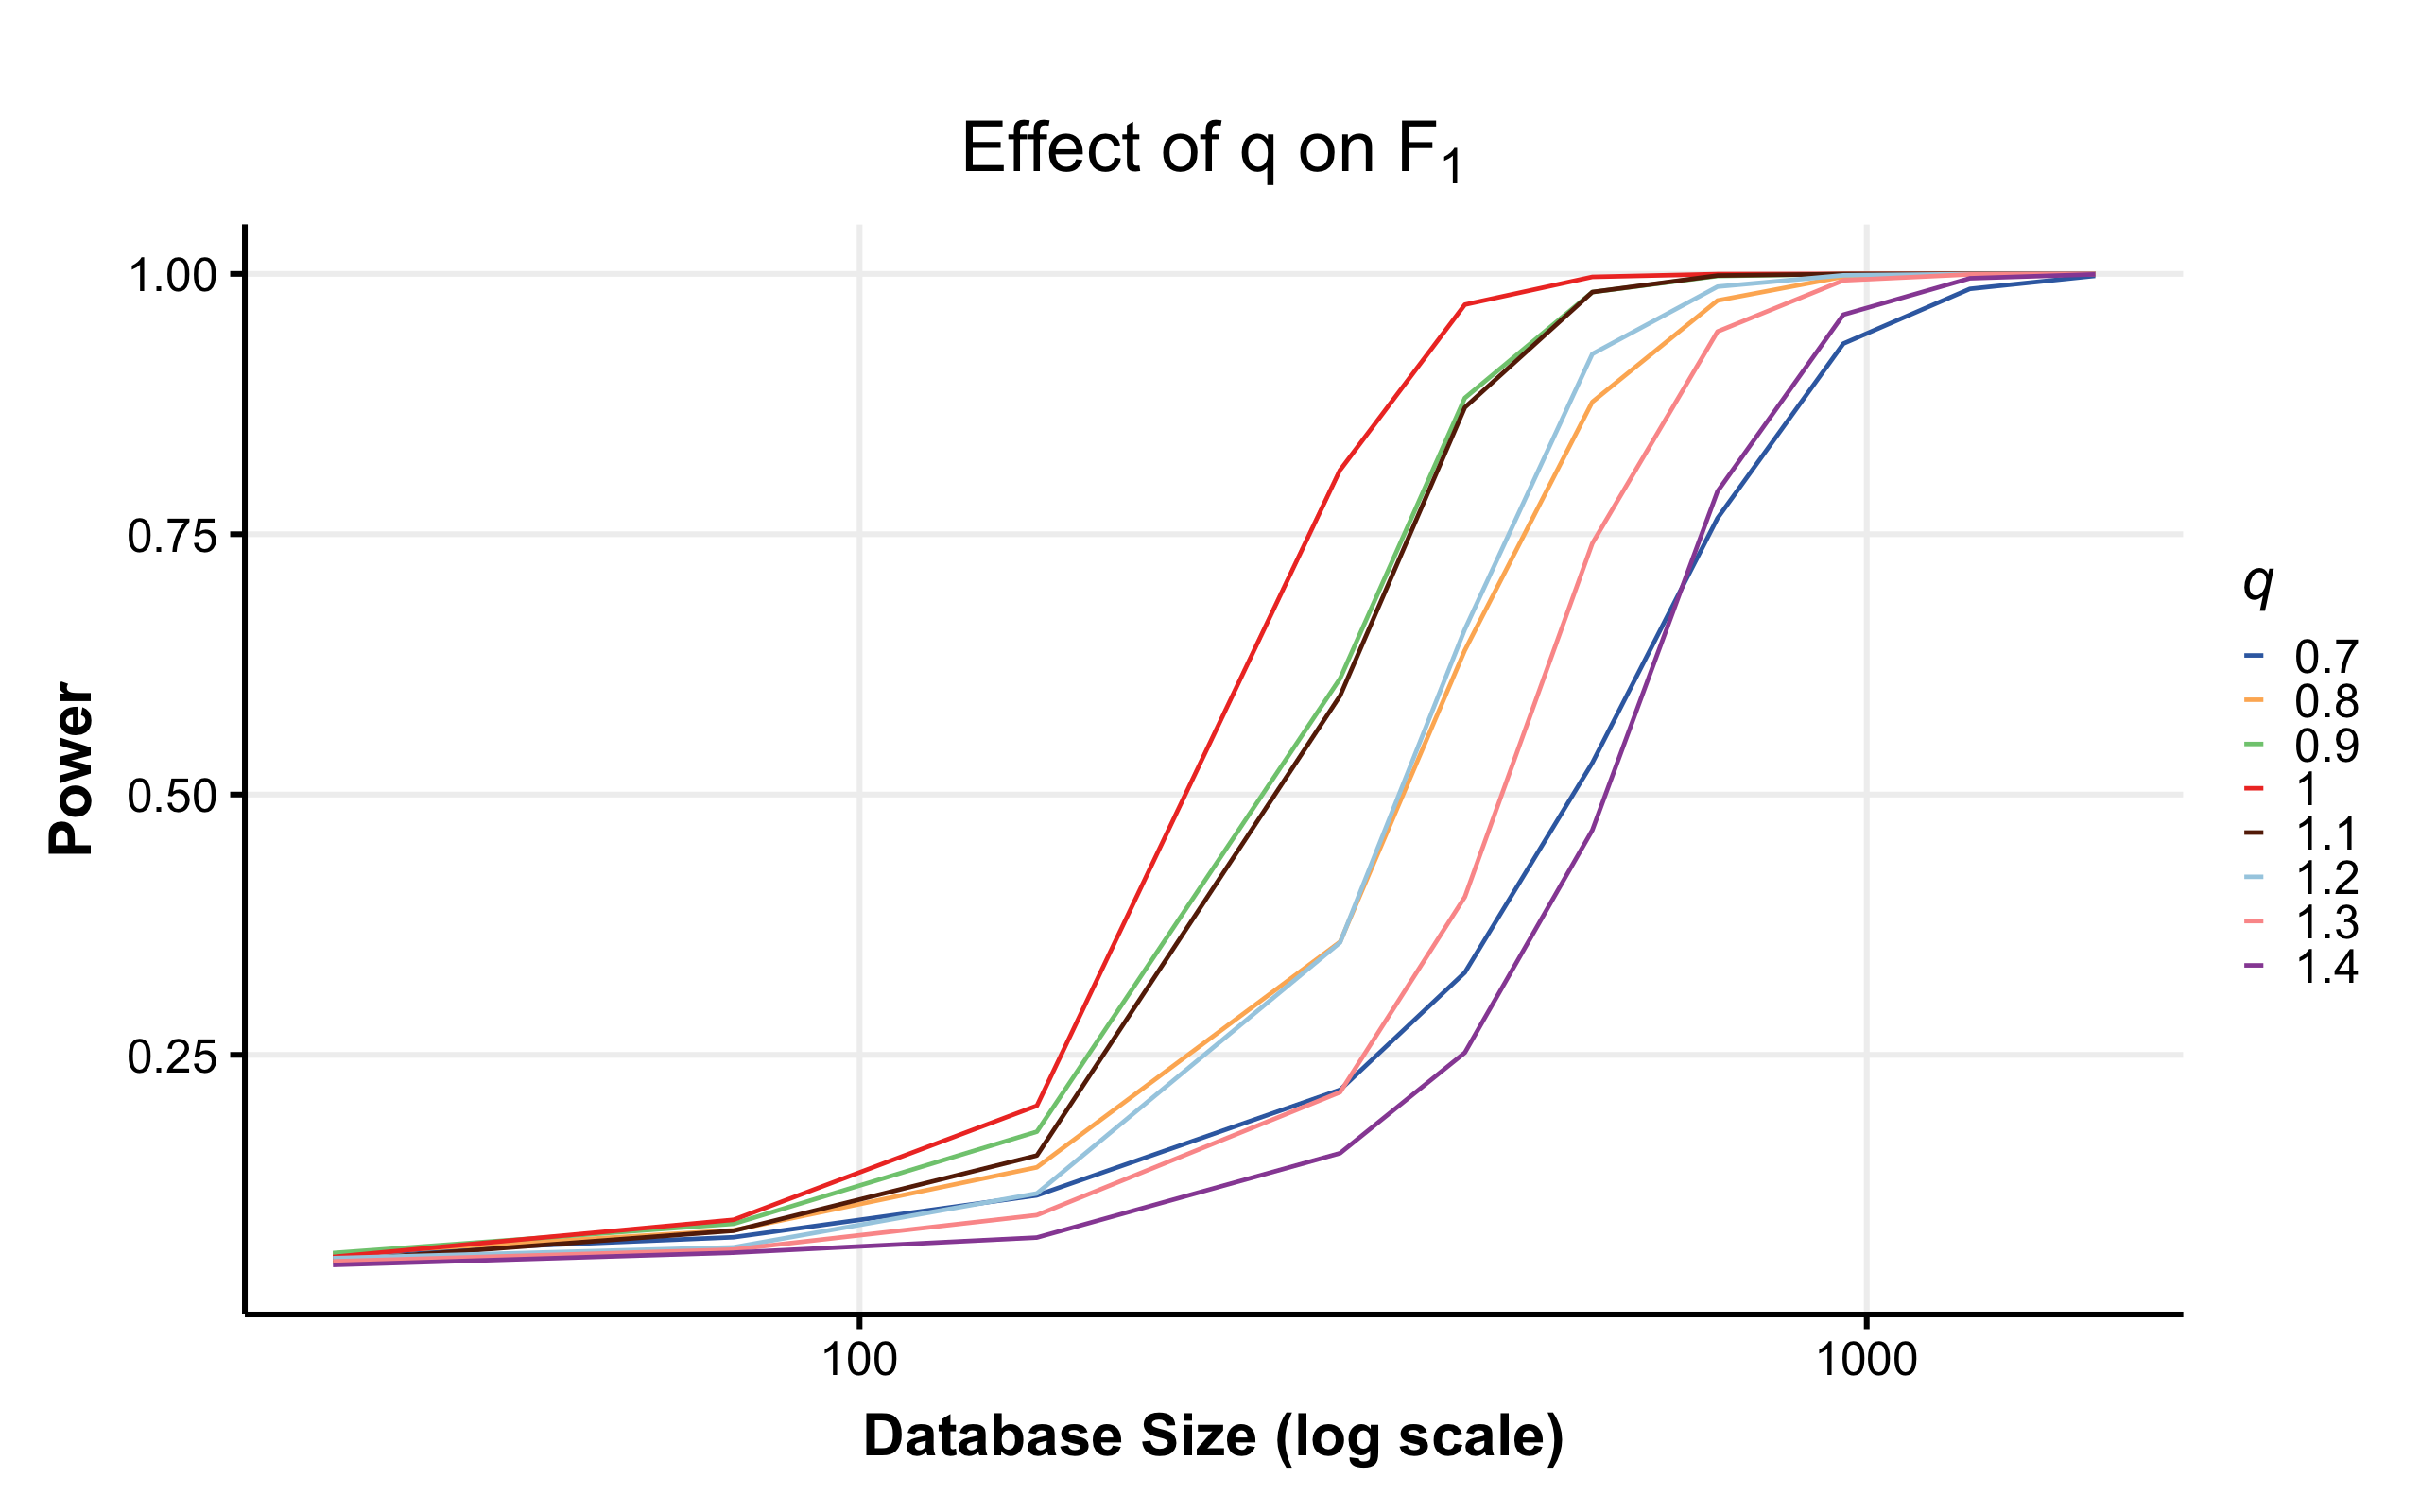
\includegraphics[width=\linewidth]{fq-power.png}
\caption{Power curves at varying exponents in a simulation setting where $k = 3$, $\sigma = .15$, and effect size: $1\sigma$. Power is experimentally maximized when $q = 1$.}\label{fig:fqpower}
\end{figure}



\subsection{Parameter tuning}\label{subsec:params}

With the generalization of the $F$-statistic, we add $q$ to the list of parameters that determine the power of a testing procedure. The parameters can be organized as follows:

\vspace{3mm}
\textbf{Data Generation:} $N$, $k$, $\sigma$, effect size \\
\indent\textbf{Private Algorithm:} $\epsilon$, $q$, $\rho$
\vspace{3mm}

The analyst gets to select the parameters corresponding to the private algorithm. While
$\epsilon$ is set based on privacy concerns, $q$ and $\rho$ should be set to 
maximize power, which our work suggest occurs at roughly 1 and 0.7, respectively.
This conclusions is based upon an extensive exploration of the parameter space, 
a selection of which can be found in Appendix~\ref{Sec:AppOptPars}.

The salient feature of these plots is that the choice of $q$ is much more 
consequential than the choice of $\rho$. In the setting where $\epsilon = .1$, 
we found that the result seen in Figure~\ref{Fig:f1-vs-f2} -- a greater than 
10-fold reduction in database size to get equivalent power -- holds across a range
of difference data generation parameters.

By contrast, the effect of $\rho$ on power is much smaller; the database size
reduction is closer to 1.1- or 1.2-fold when moving from $\rho = .5$ to $\rho = .7$
when $\epsilon = .1$.

